\chapter{Track Reconstruction}
\label{sec:track}
	As the~first step of the~reconstruction algorithm, we reconstruct the~track of a~primary particle -- either an~electron or a~positron. Then, using this information, we determine the~energy of the~particle (Section~\ref{sec:energy}).
	
	The~\textbf{Reconstruction Assuming Steady Drift} uses the~standard \ac{TPC} approach. With parallel fields, the~drift inside a~uniform electric field remains undistorted (as shown in Equation~\ref{eq:drift}). Therefore, we only need to reconstruct the~$z$\nobreakdash-coordinate from the~drift time using the~known drift velocity. We also assume that the~readout coordinates ($x'$,~$y'$,~$t$) are known exactly, neglecting the~pads and time binning.
	
	Reconstruction using an~\textbf{Ionization Electron Map} (from now on referred to as \emph{the~map}) uses a~simulation of the~drift of secondary (ionization) electrons within the~detector volume. This simulation can then be used to interpolate the~initial position of the~secondary electrons. In the~first iteration of this method the~readout is assumed to be continuous.
	
	We present two algorithms using the~map for reconstruction. The~first one uses a~gradient descent algorithm along with trilinear interpolation (see Section~\ref{sec:trilin}) of the~map. The~second method uses interpolation on the~irregular inverse grid with a~polynomial.
	
	The~\textbf{Discrete Reconstruction} uses the~map; instead of reconstructing the~exact position of each electron, we reconstruct the~center of each hit pad together with the~time corresponding to the~midpoint of the~time bin. The~electron count in each \ac{TPC}~bin (consisting of the~pad and the~time bin) serves as an~idealized collected charge, which is then used as a~weight in the~energy reconstruction fit.
	
	\section{Reconstruction Assuming Steady Drift}
	\label{sec:trackfirst}
		As the~first step, we tried to reconstruct a~simulated electron track with a~special set of initial parameters, described in detail in Section~\ref{sec:microfirst}. The~starting point is given by the~origin of our coordinate system and its initial direction is given by the~positive $x$\nobreakdash-axis. This means the~magnetic field of our detector is perpendicular to the~momentum of the~particle at all times, and we can reduce the~problem to two-dimensional space.
		
		For the reconstruction, we decided to use the~common method used in a~standard \ac{TPC}\red{~(similar to?, cite some source(s)!)}. This will allow us to explore the~significance of the~atypical behavior in our \ac{OFTPC}. Additionally, we assume the~readout is continuous to further simplify the~problem. In this approximation, we reconstruct the~initial position of each ionization electron.
		
		The~reconstruction is then defined by the~following relations between the~coordinates of the~detector space and the~readout space (see Section~\ref{sec:coor}):
			\begin{align}
				x &= x',\\
				y &= y',\\
				z &= 8\;\text{cm} - d_r = 8\;\text{cm} - v_d t,
			\end{align}
		where $d_r$ is the~distance to the~readout, and $v_d$ is the~drift velocity of electrons in the~given gas mixture. At a~phenomenological level, this velocity can be considered as a~function of the~electric field~$\bm{E}$ and the~magnetic field~$\bm{B}$ as shown in Equation~\ref{eq:drift}.\red{~The~\garfieldpp toolkit uses this fact to accelerate their drift simulation with non-microscopic approaches (could mention in the~simulation chapter).} Since we assume a~uniform electric field in the~detector and in this~approximation we want to neglect the~effect of our unusual magnetic field, we consider the~drift velocity constant. We can estimate the drift velocity by fitting the dependence $d_r(t)$ of ionization electrons from a~simulated track with a linear function:
			\begin{equation}
				d_r(t) = v_d t + d_0.
			\end{equation}
		The fit was applied on two tracks with different gas composition, the result is in Figure~\ref{fig:zt}.\red{~Compare with real drift velocities -- a good indication of the~tilt of drift lines.} The obtained parameters are then used for the reconstruction shown in Figure~\ref{fig:rasd_xz}. From the~residuals shown in Figure~\ref{fig:rasd_res}, we can see that this reconstruction algorithm leads to significant deviations from the simulated track (up to 1.1~cm for 90:10, and up to 0.3~cm for 70:30 Ar:CO$_2$), especially in the~faster gas mixture 90:10 (as expected -- for a~higher mean time between collisions in Equation~\ref{eq:drift}, the effect of the magnetic field is bigger). These deviations are mainly caused by the~shift in the $x$\nobreakdash-coordinate due to the~tilt of the drift lines in magnetic field. In order to account for this, we need to develop a~better algorithm.\red{~There is also a~small irregularity in the $z$\nobreakdash-coordinate but it is comparable with the diffusion. We can/will also later show that this has a significant effect on the reconstructed energy.}
		
		\begin{figure}
			\centering
			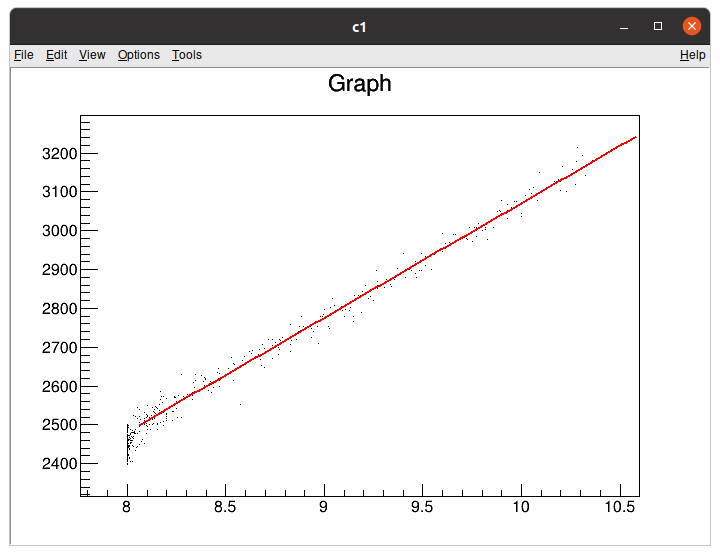
\includegraphics[width=0.48\textwidth]{9010_zt.png}
			\hfill
			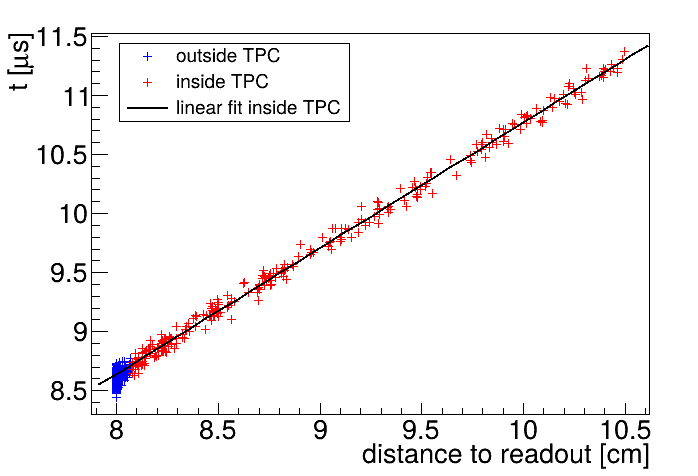
\includegraphics[width=0.48\textwidth]{7030_zt.png}
			\caption{Linear fit of the~drift time $t$ dependence on the~distance to the readout $d_r = 8\;\text{cm} - z$ for the ionization electrons in 90:10 (left) and 70:30 (right) Ar:CO$2$ gas composition. Only electrons inside the~\ac{TPC} (red) are fitted. The parameters are $v_d = \SI{3.39}{\centi\meter\per\micro\second}$, $d_0 = -0.41$~cm for 90:10, and $v_d = \SI{0.939}{\centi\meter\per\micro\second}$, $d_0 = -0.11$~cm for 70:30 Ar:CO$_2$.}
			\label{fig:zt}
		\end{figure}
		
		\begin{figure}
			\centering
			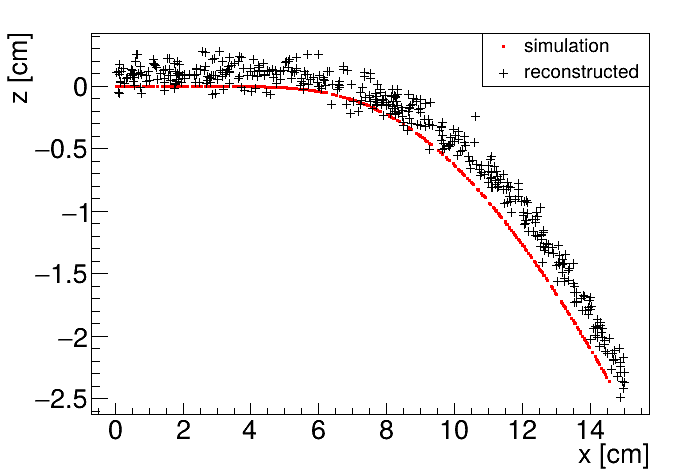
\includegraphics[width=0.48\textwidth]{9010_xz_rasd.png}
			\hfill
			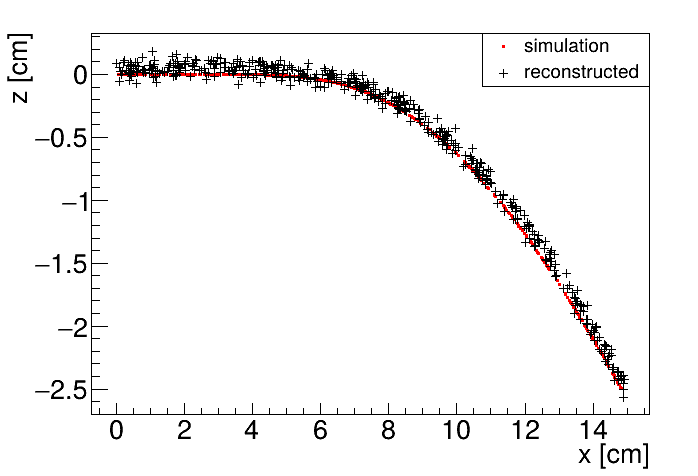
\includegraphics[width=0.48\textwidth]{7030_xz_rasd.png}
			\caption{Reconstruction (black) of the~starting position of ionization electrons (red) using parameters obtained from the~fit (Figure~\ref{fig:zt}). Two gas compositions 90:10 (left) and 70:30 Ar:CO$_2$ (right) are compared.}
			\label{fig:rasd_xz}
		\end{figure}
		
		\begin{figure}
			\centering
			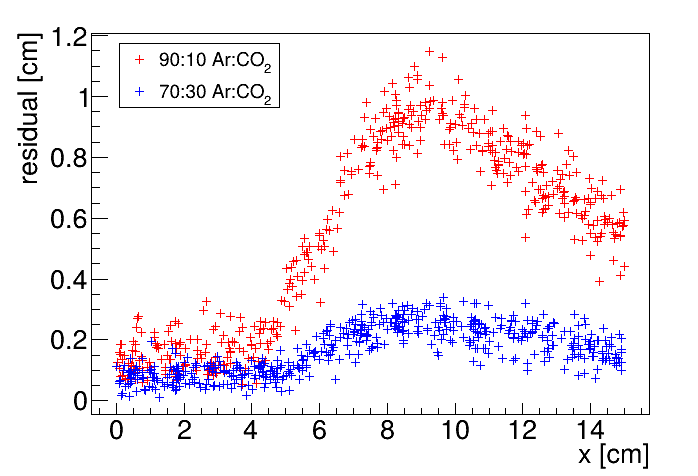
\includegraphics[width=0.7\textwidth]{rasd_res.png}
			\caption{Comparison of residuals (i.e., the distance from the reconstructed point to the simulated ionization electron starting point) dependence on~$x$ for two gas mixtures 90:10 (red) and 70:30 Ar:CO$_2$ (blue).}
			\label{fig:rasd_res}
		\end{figure}
	
	\section{Ionization Electron Map}
	\label{sec:map}
		Inside an~\ac{OFTPC}\orange{~($\exists$ more than one, also considering it a~general concept rather than the specific OFTPC used at this experiment)}, the~drift of the~ionization electrons is significantly affected by its magnetic field as shown in Equation~\ref{eq:drift}, see also Figure~\ref{fig:microfirst}. We need to take this into account for accurate reconstruction\red{~(should be easy to run the~reconstruction without the map and show how much it improves the results)}. In the~first approximation, we assume a~continuous readout (i.e., we neglect the~anode segmentation into pads). We can then reconstruct the~original position of each ionization electron using its readout coordinates. For this purpose, we use the~ionization electron map.
		
		The~ionization electron map represents a~mapping from the~detector space to the~readout space (see Section~\ref{sec:coor}). It tells us what readout coordinates $(x',y',t)$ we can expect on average for an~ionization electron created at the~detector coordinates $(x,y,z)$. More precisely, it is a~mapping to the~distributions on the~readout space; we can simplify this as only the means $\overline{\mathcal{M}}$ and the covariance matrices $\mathcal{M}_\mathbf{\Sigma}$, assuming Gaussian distribution:
			\begin{alignat}{3}
				\overline{\mathcal{M}}&\colon \mathcal{D} \longrightarrow \mathcal{R}, &&(x,y,z) \longmapsto \mathbf{\overline{X}}^T\equiv(\bar{x}',\bar{y}',\bar{t}),\\
				\mathcal{M}_\mathbf{\Sigma}&\colon \mathcal{D} \longrightarrow \mathbb{R}^{3\times3}, &&(x,y,z) \longmapsto \mathbf{\Sigma}^{\phantom{T}} \equiv \scalebox{0.9}{$\begin{pmatrix}
					\sigma_{x'}^2 & \operatorname{cov}(x',y') & \operatorname{cov}(x',t) \\
					\operatorname{cov}(y',x') & \sigma_{y'}^2 & \operatorname{cov}(y',t) \\
					\operatorname{cov}(t,x') & \operatorname{cov}(t,y') & \sigma_{t}^2
				\end{pmatrix}$},\\
				\mathcal{M}&\colon \mathcal{D} \longrightarrow D(\mathcal{R}),\ &&(x,y,z) \longmapsto N(\mathbf{X}) \equiv \frac{\exp(-\frac{1}{2}(\mathbf{X}-\mathbf{\overline{X}})^T\mathbf{\Sigma}(\mathbf{X}-\mathbf{\overline{X}}))}{\sqrt{(2\pi)^3 |\mathbf{\Sigma}|}}.
			\end{alignat}
		To get an~approximation of this mapping, we simulate the~drift of ionization electrons generated on a~regular Cartesian grid $\mathbb{G}\subset\mathcal{D}$ with spacing~$l$ inside the~volume of our \ac{OFTPC}\footnote{The~detector walls are not considered and we simulate the~drift even outside of the~\ac{OFTPC} which allows us to interpolate even close to the~walls} (see the visualization in Figure~\ref{fig:map_3d}). In Figure~\ref{fig:maplines}, you can see an example of drift lines from a~test of the~simulation. After testing runs, two map simulations were made with different gas composition, their parameters are shown in Table~\ref{tab:map}. 
		
		\begin{figure}
			\centering
			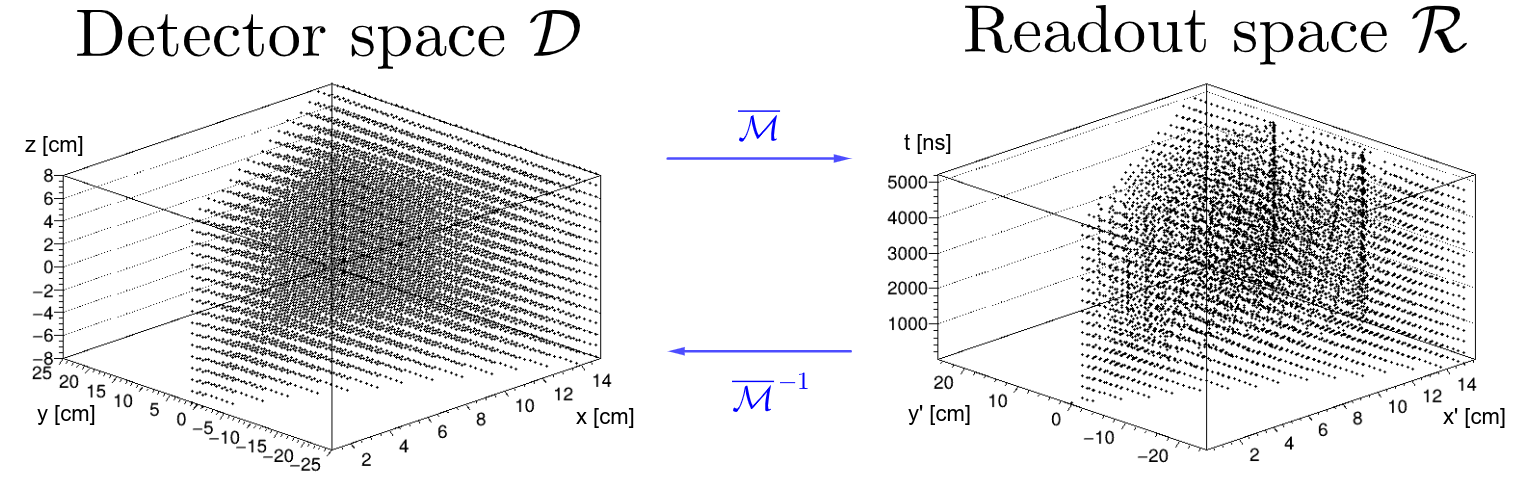
\includegraphics[width=\textwidth]{map_3dvis.png}
			\caption{A~3D visualization of the mapping of means $\overline{\mathcal{M}}$ for the 90:10 Ar:CO$_2$ gas. A regular grid $\mathbb{G}$ with $l = \SI{1}{\centi\meter}$ in the detector space is mapped to an~irregular grid $\mathbb{G}^{-1} \equiv \overline{\mathcal{M}}(\mathbb{G})$ in the readout space.}
			\label{fig:map_3d}
		\end{figure}
		
		\begin{figure}
			\centering
			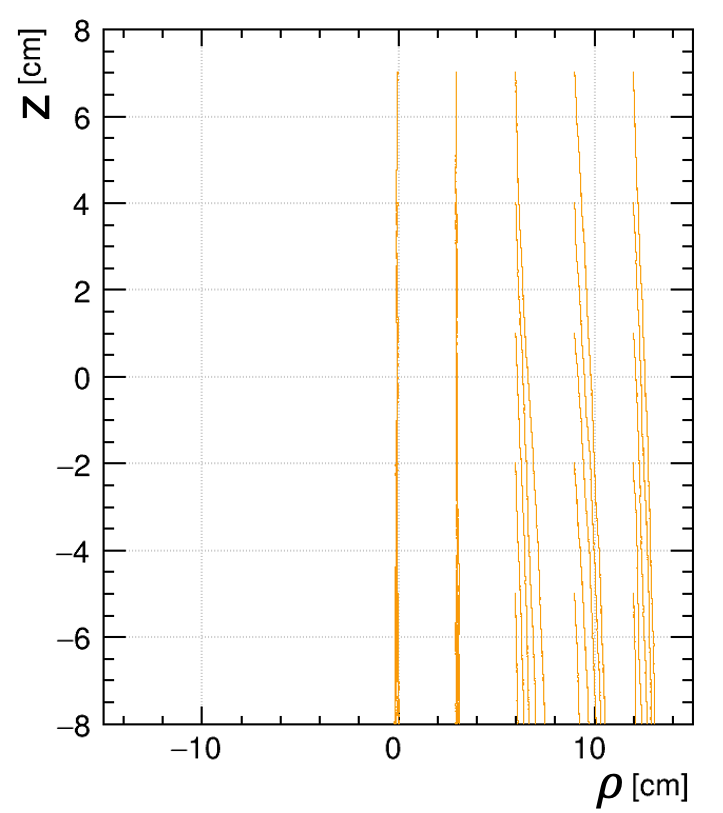
\includegraphics[width=0.5\textwidth]{map_lines.png}
			\caption{A test of the 90:10 Ar:CO$_2$ map simulation with spacing $l = \SI{1.5}{cm}$. The resulting drift lines of evenly spaced electrons are displayed in orange.}
			\label{fig:maplines}
		\end{figure}
		
		\begin{table}
			\centering
			\caption{Comparison of parameters of two map simulations.}
			{\renewcommand{\arraystretch}{1.2}
			\begin{tabular}{|c|c|c|}
				\hline
				\textbf{Parameter} & \textbf{90:10 Ar:CO$_2$ map} & \textbf{70:30 Ar:CO$_2$ map}\\
				\hline
				$N$ & 100 & 100 \\
				\hline
				$l$ & 1.0 cm & 0.5 cm \\
				\hline
				$z$ bounds & $[-8,8]$ cm & $[-8,8]$ cm \\
				\hline
				$x$ bounds & $[0,15]$ cm & $[-1.5,15.0]$ cm \\
				\hline
				$y$ bounds & $|y| \leq x\cdot\tan\frac{\pi}{3}$ & $|y| \leq (x+\SI{1.5}{\centi\meter})\cdot\tan\frac{\pi}{6}$ \\
				\hline
			\end{tabular}}
			\label{tab:map}
		\end{table}
		
		In order to get accurate results, we use the~microscopic simulation of these electrons described in Section~\ref{sec:microsim}\red{~(Monte Carlo from \textit{AvalancheMC} was also considered but it doesn't (didn't? CERES used it from MAGBOLTZ???) include magnetic field, we can probably improve this anyway using the fast track simulation with map proposed in the future section)}. It is also useful to simulate multiple~($N$) electrons originating from the~same position so that we can account for the~random fluctuations due to collisions. Using the readout coordinates of the~electrons, we then estimate the means and the covariance matrix:
			\begin{equation}
				\label{eq:cov}
				\mathbf{\overline{X}} = \frac{1}{N}\sum_{i=1}^{N} \mathbf{X}_i,\qquad \mathbf{\Sigma} = \frac{1}{N-1}\sum_{i=1}^{N}(\mathbf{X}_i-\mathbf{\overline{X}})(\mathbf{X}_i-\mathbf{\overline{X}})^T,
			\end{equation}
		where $\mathbf{X}_i$ represents the readout coordinates $(x'_i, y'_i, t_i)^T$ of the $i$\nobreakdash-th electron. The matrix (resp. its submatrix) can then be used to plot error ellipsoid (resp. ellipse). The axes correspond to the eigenvectors, errors along these axes for a~given confidence level~$p$ can be computed using the chi\nobreakdash-squared distribution
			\begin{equation}
				\label{eq:sigma}
				\sigma_i = \sqrt{\lambda_i \chi^2_k(p)},
			\end{equation}
		where $\lambda_i$ is the corresponding eigenvalue and $k$~is the~number of degrees of freedom.
		
		As shown in \cref{fig:map_zt,fig:map_xt}, the drift times in the map are no longer proportional to the $z$\nobreakdash-coordinate due to the varying Lorentz angles in the inhomogeneous magnetic field (see Equation~\ref{eq:lorentz}). As expected, the effect is considerably larger in gases with higher drift velocities. Similarly, the drift distortion (i.e., its deviation from the vertical lines) is huge for the "faster" gas, but still significant for the "slower" one, as demonstrated in \cref{fig:map_yx_all,fig:map_bot,fig:map_xz}.
		
		\begin{figure}
			\centering
			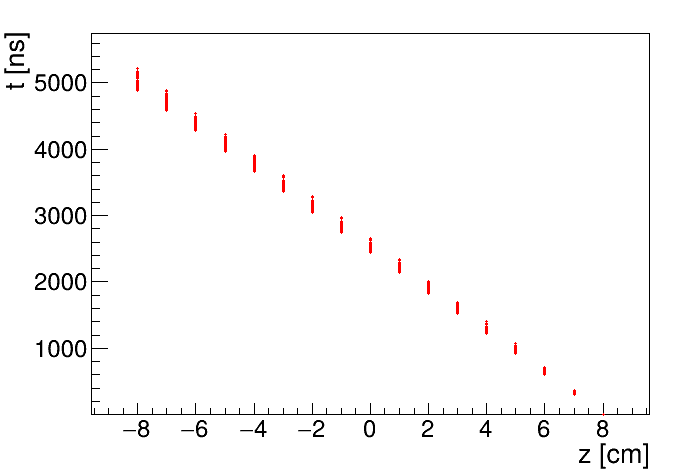
\includegraphics[width=0.48\textwidth]{map_zt_9010.png}
			\hfill
			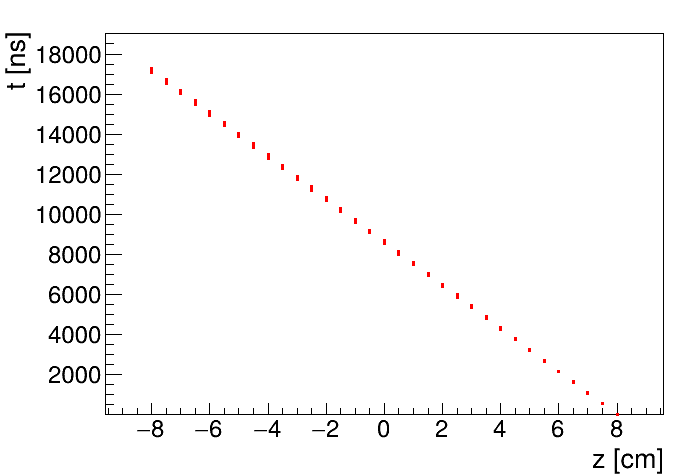
\includegraphics[width=0.48\textwidth]{map_zt_7030.png}
			\caption{Dependence of the drift times of the simulated map $\overline{\mathcal{M}}$ on the $z$\protect\nobreakdash-coordinate. Two gas mixtures 90:10 (left) and 70:30 Ar:CO$_2$ (right) are compared. The spread is caused by varying Lorentz angles.}
			\label{fig:map_zt}
		\end{figure}
		
		\begin{figure}
			\centering
			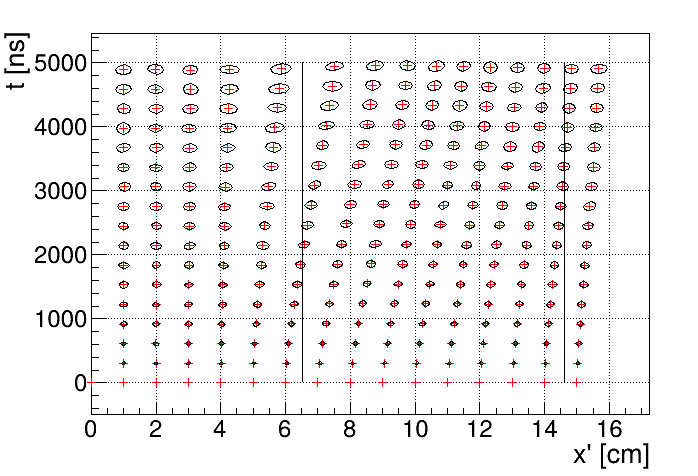
\includegraphics[width=0.48\textwidth]{map_xt_9010.png}
			\hfill
			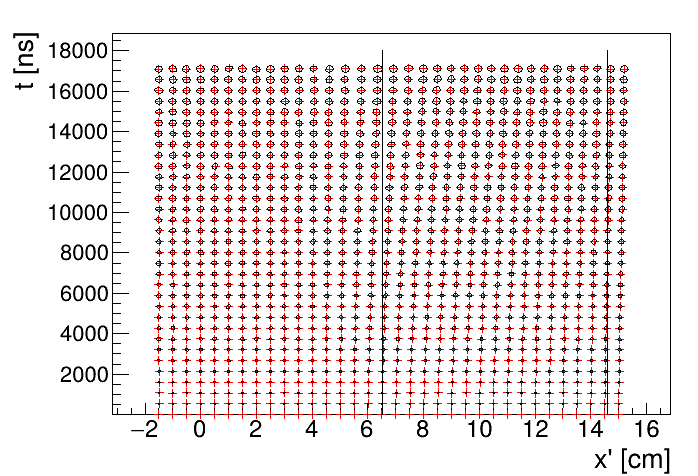
\includegraphics[width=0.48\textwidth]{map_xt_7030.png}
			\caption{The $x't$ projection of the $\mathcal{M}(\mathbb{G}_{y=0})$ mapping of a~part of the~regular grid $\mathbb{G}$. The means $\overline{\mathcal{M}}(\mathbb{G}_{y=0})$ are marked with red crosses, and the diffusion error is denoted by black 95\% confidence error ellipses computed from the diagonalized covariance matrices $\mathcal{M}_{\mathbf{\Sigma}}(\mathbb{G}_{y=0})$. Two gas mixtures 90:10 (left) and 70:30 Ar:CO$_2$ (right) are compared. The first mixture shows differences of~$t$ for electrons with same initial~$z$ but different initial~$x$. For the second mixture, these differences are negligible in comparison with the diffusion.}
			\label{fig:map_xt}
		\end{figure}
		
		\begin{figure}
			\centering
			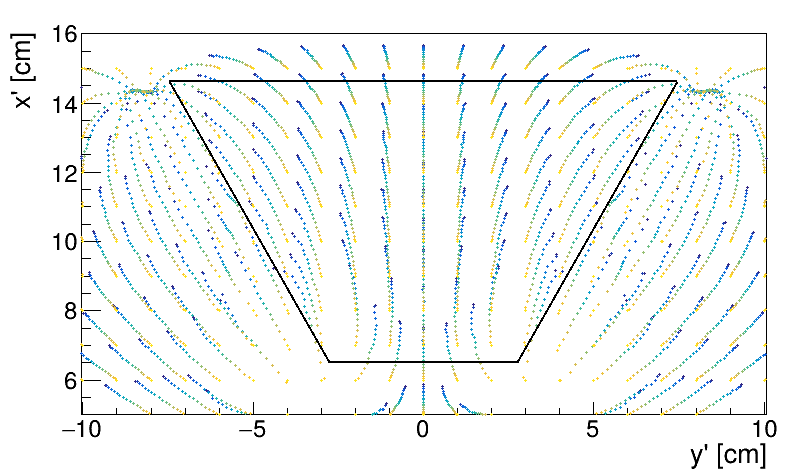
\includegraphics[width=0.48\textwidth]{map_yx_all_9010.png}
			\hfill
			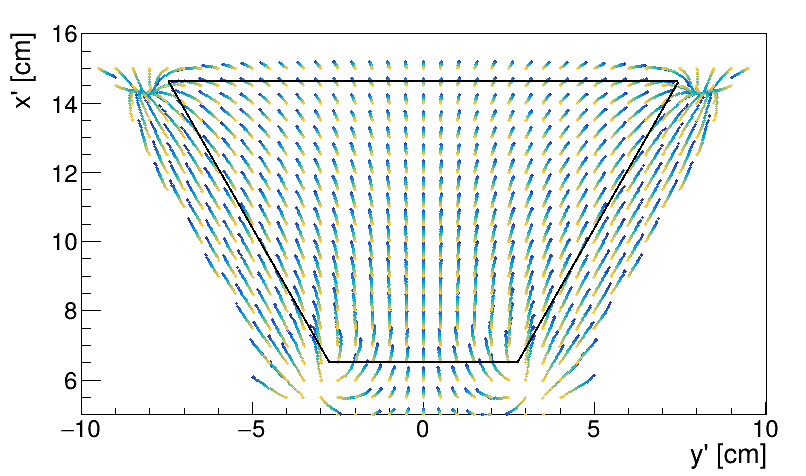
\includegraphics[width=0.48\textwidth]{map_yx_all_7030.png}
			\caption{The regular grid $\mathbb{G}$ projected by the mapping $\overline{\mathcal{M}}$ from the detector space onto the $x'y'$~plane ($t$ is not plotted). Layers with lower $z$\protect\nobreakdash-coordinate (i.e., further away from the readout) are displayed with darker colors. The~\ac{OFTPC} volume is marked with black lines. Two gas mixtures 90:10 (left) and 70:30 Ar:CO$_2$ (right) are compared.}
			\label{fig:map_yx_all}
		\end{figure}
		
		\begin{figure}
			\centering
			\begin{subfigure}[t]{\textwidth}
				\centering
				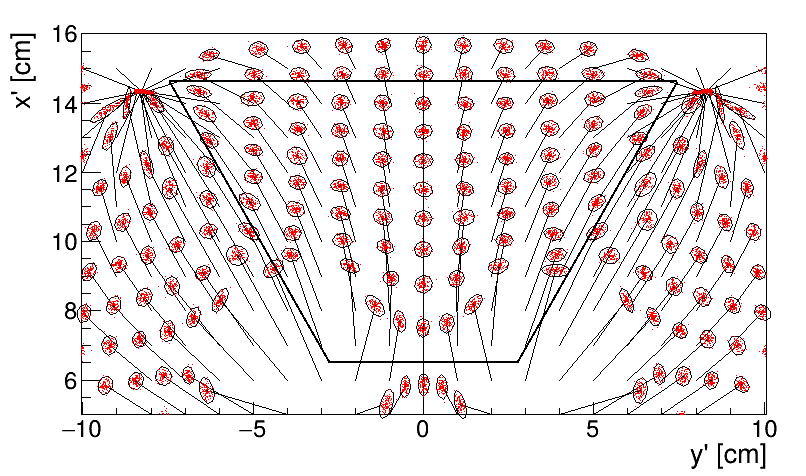
\includegraphics[width=0.48\textwidth]{map_yx_bottom_9010.png}
				\hfill
				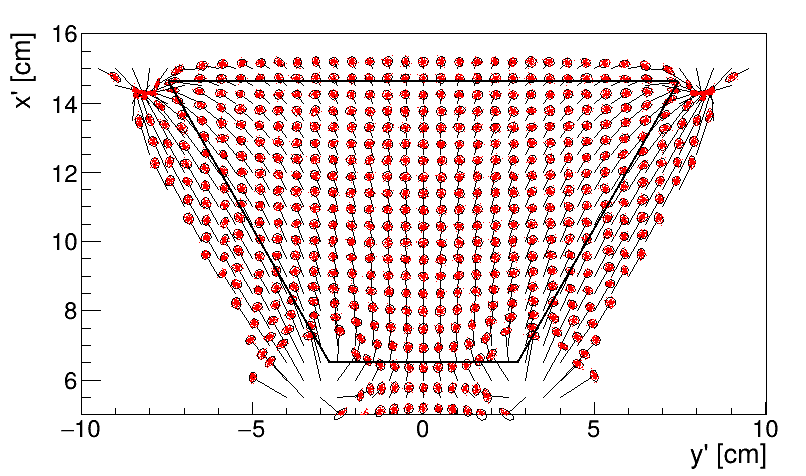
\includegraphics[width=0.48\textwidth]{map_yx_bottom_7030.png}
				\caption{The $x'y'$ projection of $\mathcal{M}(\mathbb{G}_{-8})$ (similar as in Figure~\ref{fig:map_yx_all}), the diffusion is denoted with the 95\% error ellipses from  the diagonalized sample covariance matrices $\mathcal{M}_\mathbf{\Sigma}(\mathbb{G}_{-8})$ $\leftrightarrow$ Equation~\ref{eq:cov}, and computed using Equation~\ref{eq:sigma}. The mean values $\overline{\mathcal{M}}(\mathbb{G}_{-8})$ are connected by black arrows with the corresponding starting position $(x,y)$ of the simulated electrons. The~\ac{OFTPC} volume is marked with black lines.}
				\label{fig:map_yx_bot}
			\end{subfigure}
			
			\begin{subfigure}[t]{\textwidth}
				\centering
				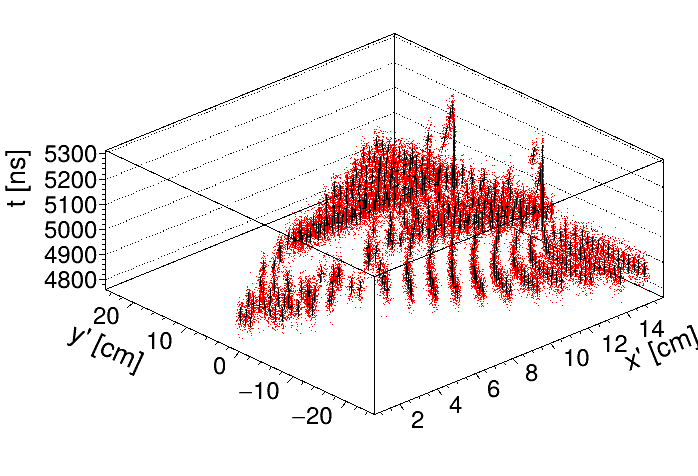
\includegraphics[width=0.48\textwidth]{map_xyt_9010.png}
				\hfill
				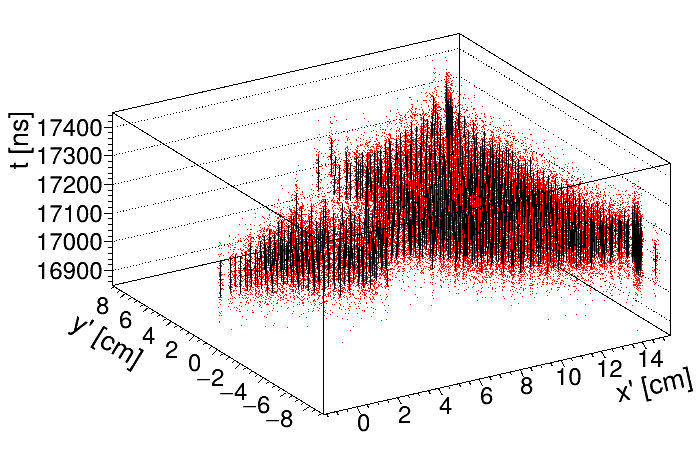
\includegraphics[width=0.48\textwidth]{map_xyt_7030.png}
				\caption{The full mapping $\mathcal{M}(\mathbb{G}_{-8})$, the diffusion is marked using standard error bars (black) from the diagonalized sample covariance matrices (Equations~\ref{eq:cov} and~\ref{eq:sigma}).}
				\label{fig:map_xyt}
			\end{subfigure}
			\caption{The $\mathcal{M}(\mathbb{G}_{-8})$ mapping of the~bottom ($z = \SI{-8}{\centi\meter}$) layer $\mathbb{G}_{-8}$ of the regular grid $\mathbb{G}\subset\mathcal{D}$. It includes both the~mapping of means $\overline{\mathcal{M}}$ and of covariances $\mathcal{M}_\mathbf{\Sigma}$. Individual electrons from the map simulation are marked with red dots. Two gas mixtures 90:10 (left) and 70:30 Ar:CO$_2$ (right) are compared.}
			\label{fig:map_bot}
		\end{figure}
		
		\begin{figure}
			\centering
			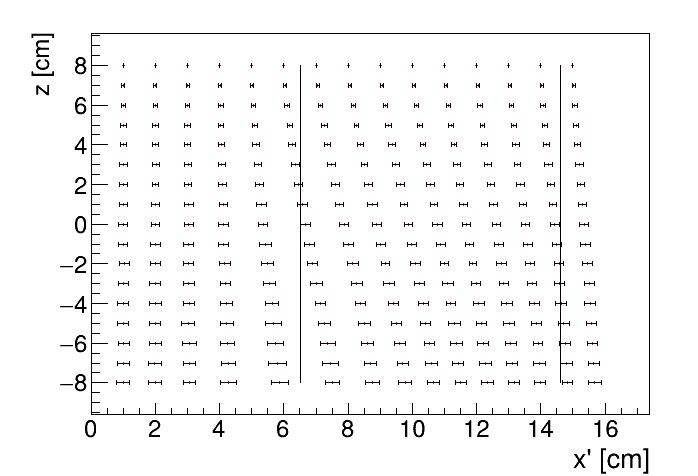
\includegraphics[width=0.48\textwidth]{map_xz_9010.png}
			\hfill
			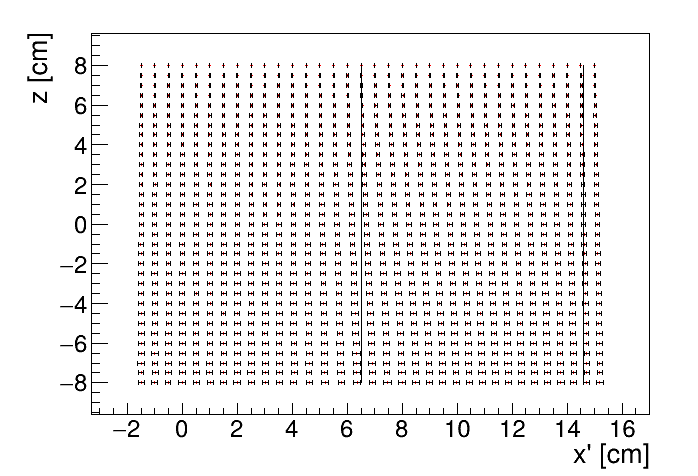
\includegraphics[width=0.48\textwidth]{map_xz_7030.png}
			\caption{The readout coordinate~$x'$ for points on the grid $\mathbb{G}_{y=0}$ plotted against their initial coordinate $z$. The means are marked with red crosses, the diffusion in~$x'$ is denoted by standard error bars. Two gas mixtures 90:10 (left) and 70:30 Ar:CO$_2$ (right) are compared.}
			\label{fig:map_xz}
		\end{figure}
		
		When evaluating the~map inside the~grid, we use trilinear interpolation (see Section~\ref{sec:trilin}). From now on, we will use the~same symbol $\mathcal{M}$ for this interpolated simulation.
		
		Finally, we need to invert the~map to get the~original detector coordinates $(x,y,z)$ from the~given readout coordinates $(x',y',t)$. In our case, it is reasonable to assume that the mapping $\overline{\mathcal{M}}$\red{~(we lose the information about the~distribution (a~wild idea how to recover this is in the Future section but it will only make sense if the~GEM is already accounted for and is very preliminary as there are many factors to consider))} is one-to-one (as seen in the simulations). We implemented two methods for this purpose: the gradient descent search (Section~\ref{sec:grad}) and interpolation on the~inverse grid (Section~\ref{sec:interpol}).
		
		The~simulation\orange{~(?)} of the~map is a~computationally heavy task. For this reason, we use the~MetaCentrum grid~\cite{metacentrum} to parallelize needed calculations. At first, this was done by evenly distributing the~simulated electrons across the~individual jobs in a~simulation with only one electron per vertex in the~regular grid~$\mathbb{G}$ with a~spacing of one centimeter. Later, a~more efficient approach was implemented, accounting for the~varying lengths of the~drift of individual electrons. If we index the~vertices of~$\mathbb{G}$ in the~order of increasing coordinates $y,x,z$\red{~(picture will make things clearer)}, we can express the~number~$n_l$ of full XY~layers (i.e., electrons with the~same $z$~coordinate, the mapping of one such layer is shown in Figure~\ref{fig:map_xyt}) with index less than or equal to $i$
			\begin{equation}
				n_l(i) = \left\lfloor\frac{i}{n_{xy}}\right\rfloor,
			\end{equation}
		where $n_{xy}$ is the~number of electrons in each XY~layer calculated simply by counting the~electrons that satisfy boundary conditions for $x$~and~$y$.\red{~These conditions should be mentioned above; sector condition + maximal $x$ value.} The~number of electrons remaining in the~top layer is then
			\begin{equation}
				n_r(i) = i\!\!\!\!\mod n_{xy}.
			\end{equation}
		Finally, we can calculate the~sum of the~drift gaps of electrons up to index~$i$
			\begin{equation}
				d_\text{sum} = (z_\text{max}-z_\text{min})n_{xy}n_l-\frac{n_l(n_l-1)}{2}n_{xy}l+n_r(z_\text{max}-z_\text{min}-n_l l).
			\end{equation}
		We then use a~binary search algorithm to find the~maximum index $i$ such that the value of this sum is less than the~fraction $\frac{\text{job id}}{\text{max job id}}$ of the~total sum. This way we obtain the~minimal and the~maximal index of electrons simulated in the~given job.
		\red{Picture of the~simulating grid (1 layer). zmin zmax also}
		
		\red{The~obtained map is then stored in a~custom class template \textit{Field}, could expand on that. Maybe earlier, since the~same template is used for the~magnetic field.}
		
		\red{Simulation inside of one sector (at first double angle). Extra space on the~sensor. Using qsub (not sure if important). Add plots of distortion of the~coordinates.\\}
		
		\noindent\red{Images to add (comparison of both simulations):
		\begin{itemize}[topsep=4pt,itemsep=2pt]
			\item Already have a simple 2D map visualization from the RD51 presentation, can use it or make something better
			\item $z$ vs. $t$ plot
			\item XY plane distortion for different $z$ values; with arrows and error bars, for all $z$-layers with different colors
			\item XZ plane ($y = 0$) distortion in $x$ (maybe not necessary?)
			\item XT plot ($y = 0$) showing (small) distortion in drift times\\
		\end{itemize}}
		
		\noindent\red{More images:}
		\begin{itemize}[topsep=4pt,itemsep=2pt]
			\item \red{Residuals of the~continuous readout reconstruction.}
		\end{itemize}
		
		\begin{figure}[H]
			\centering
			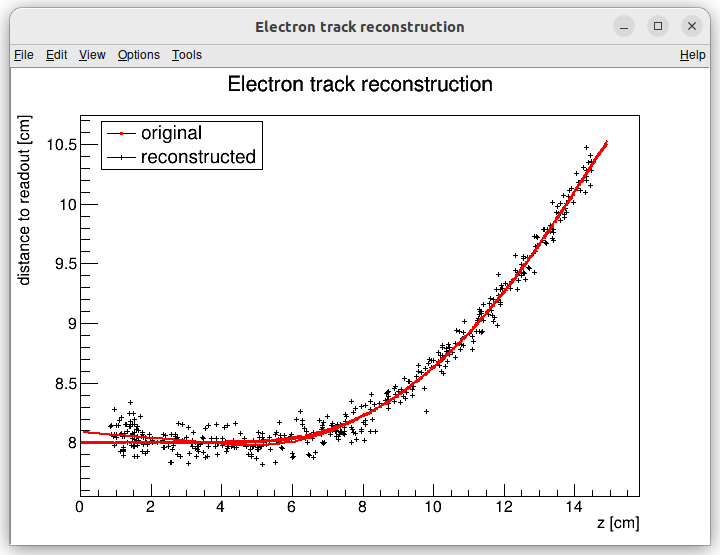
\includegraphics[width=0.5\textwidth]{9010_reco.png}
			\caption{Example reconstruction with the~map.\red{~Swap for better image, correct coordinates.}}
			\label{fig:9010reco}
		\end{figure}
		
		\subsection{Gradient Descent Algorithm}
		\label{sec:grad}			
			The~first implemented method of reconstruction uses a~gradient descent algorithm to calculate an~inversion of the~map $\overline{\mathcal{M}}$ in a~given point. Gradient descent is an~iterative minimization algorithm for multivariate functions. Let $R\in\mathcal{R}$ be a~point in the~readout space; we want to find a~point $D = (x,y,z) \in\mathcal{D}$ in the~detector space such that 
				\begin{equation}
					\overline{\mathcal{M}}(D) = R = (x'_R,y'_R,t_R).
				\end{equation}
			We define a~function~$f_R$ in the~readout space as a~distance in this space:
				\begin{equation}
					f_R(x',y',t) = \sqrt{(x'-x'_R)^2+(y'-y'_R)^2+v_d^2(t-t_R)^2},
				\end{equation}
			where $v_d$ is an~approximation of the~drift velocity in the~\ac{TPC}, obtained from the~reconstruction in Section~\ref{sec:trackfirst}\red{~(there will be an image with the~linear fit here)}. We make an~initial guess\red{~(actually in the~original code we just take $z=0$)}:
				\begin{equation}
					D_0 = (x'_R,y'_R,v_dt).
				\end{equation}
			Assuming we have the $n$-th estimate $D_n$, we calculate the~$i$-th component of the~gradient of $f_R\circ\overline{\mathcal{M}}$ numerically using central differences:\orange{~(signs look correct)}
				\begin{equation}
					\left[\nabla(f_R\circ\overline{\mathcal{M}})\right]^i(D_n) \approx \frac{f_R(\overline{\mathcal{M}}(D_n+s\cdot e^i))-f_R(\overline{\mathcal{M}}(D_n-s\cdot e^i))}{2s},
				\end{equation}
			where $e^i\in\mathcal{D}$ is the~$i$-th coordinate vector and $s$ is the~step size. The~step size should be sufficiently small; initially, we set it as a~fraction $s = \frac{l}{10}$ of the~map's grid spacing $l$. During the~minimization, we check that $f_R(\overline{\mathcal{M}}(D_n))<10s$ at all times\orange{~($s$ can (?) change -- check)}.\red{~When using trilinear interpolation, it would be more efficient to calculate the~gradient explicitly ($\pm$ same result). This could be implemented inside the~\textit{Field} template class.} The~next iteration can be calculated as follows:
				\begin{equation}
					D_{n+1} = D_n - \gamma \nabla(f_R\circ\overline{\mathcal{M}})(D_n),
				\end{equation}
			where $\gamma\in\mathbb{R}^+$ is the~damping coefficient. It should be set to a~small enough value to ensure convergence, but large enough for sufficient converging speed. The~minimization stops either when the error $f_R(\overline{\mathcal{M}}(D_n))$ drops below a~specified value or when the~number of iterations exceeds a~certain limit (in this case, a~message is printed into the~console).
			The parameters of this method can be further optimized (e.g., a~better choice of $\gamma$,\red{~gradient computation}); instead, we later decided to use the~interpolation on the~inverse grid described in the~next section.
			
			\red{Measure reconstruction duration and compare it with the~inverse grid interpolation? Also compare the~result? Typical evolution of $D_n$ during search. Not sure if this has to be cited.}
		
		\subsection{Interpolation on the~Inverse Grid}
		\label{sec:interpol}			
			\red{Interpolation should be generally faster than the~gradient descent since we don't need to iterate. We also don't need to optimize it to improve performance, if it's too slow we can even calculate the~coefficients for the~entire map before reconstruction (again, do some profiling).}
			
			The~best current algorithm uses the~interpolation on the~inverse grid. Rather than inverting the~trilinearly interpolated map using a~numerical minimization method as in the~previous section, we take advantage of the~fact that the~map $\overline{\mathcal{M}}$ is one-to-one\orange{~(isomorphism is supposed to preserve structure, not sure how to interpret that here, }\red{not the best description, we already (kind of) assume it is a~bijection by saying we will invert it)}. Since we have simulated values of this map on a~regular grid in the~detector space $\mathcal{D}$, we also know the~inverse map $\overline{\mathcal{M}}^{-1}$ on the~irregular inverse grid in the~readout space $\mathcal{R}$. To get an~approximation of the~inverse map in the~entire readout space, we can use interpolation\orange{~(general concept, the specific choice is described below)}.
			
			Since the~inverse grid is irregular, trilinear interpolation cannot be applied. Given that the~simulated map is dense enough to provide a~good approximation considering the~size of our pads, we can adopt a~similar approach.\footnote{A more complicated and computationally heavy alternative would be natural neighbor interpolation or Kriging.} As shown in Equation~\ref{eq:trilinpoly} in Section~\ref{sec:trilin}, trilinear interpolation\orange{~(shouldn't need an article when talking about a~general concept)} can be expressed as a~polynomial:
				\begin{equation}
					\widehat{f}(x,y,z) = axyz + bxy + cxz + dyz + ex + fy + gz + h,
				\end{equation}
			where $a,b,c,d,e,f,g,h$ are coefficients uniquely determined by the~values of the~function at the~vertices of the~interpolation cell\orange{~(can be calculated in the way shown in the mentioned equation, not sure what more to add)}. We can generalize this for a~function defined on an~irregular grid. Given the~function values at any eight points, we can write a~system of eight linear equations
				\begin{equation}
					\begin{pmatrix}
						x_1 y_1 z_1 & x_1 y_1 & x_1 z_1 & y_1 z_1 & x_1 & y_1 & z_1 & 1\\
						\vdots & \vdots & \vdots & \vdots & \vdots & \vdots & \vdots & \vdots\\
						x_8 y_8 z_8 & x_8 y_8 & x_8 z_8 & y_8 z_8 & x_8 & y_8 & z_8 & 1
					\end{pmatrix}
					\begin{pmatrix}
						a\\
						\vdots\\
						h
					\end{pmatrix}
					=
					\begin{pmatrix}
						f(x_1,y_1,z_1)\\
						\vdots\\
						f(x_8,y_8,z_8)
					\end{pmatrix},
				\end{equation}
			which has a~unique solution for the~coefficients for most values of $(x_n, y_n, z_n)$ and $f(x_n,y_n,z_n)$, where $n\in\{1,\ldots,8\}$.
			
			This approach introduces a~small complication: finding the~correct pseudocell (i.e., the image of eight vertices forming a~cubic cell in the~regular grid) in the~inverse grid. The~eight irregularly spaced vertices of this pseudocell do not define a~unique volume, so there are multiple possible ways to partition $\mathcal{R}$ into pseudocells, with no obvious choice among them.
			
			\red{We are currently ignoring this problem and performing binary search along $x$, $y$, $z$ (in this order). It shouldn't matter too much because the~70/30 map doesn't cause such a big distortion and was even accidentally extrapolated for all $z$ different from the central plane.}
			
			\begin{figure}[H]
				\centering
				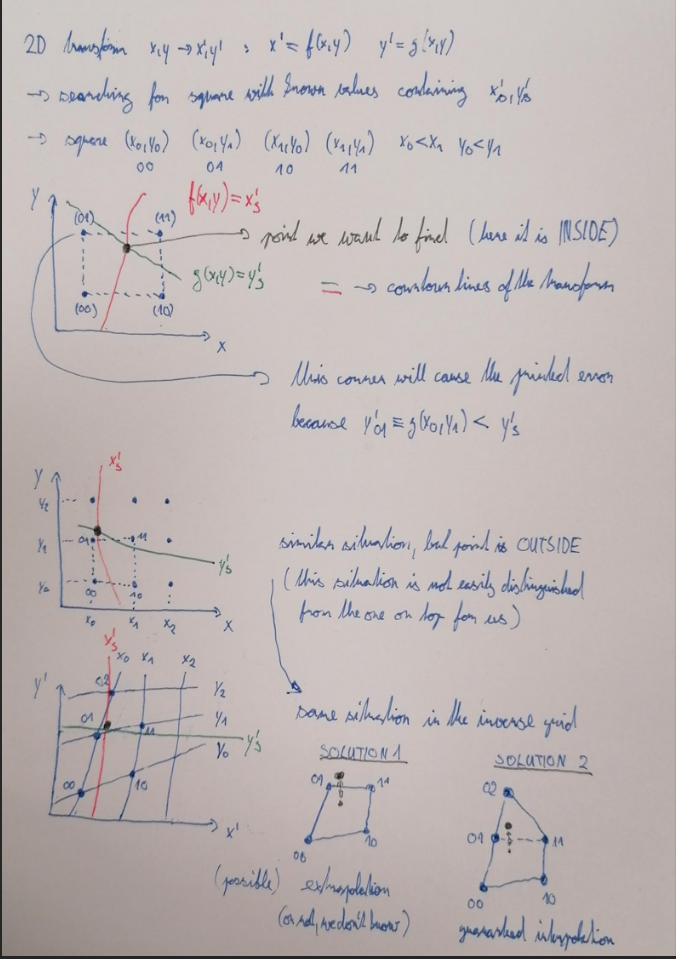
\includegraphics[width=0.8\textwidth]{interpol.png}
				\caption{Selection of the~points for interpolation.\red{~Create better images; use the~explanation interpolation vs. extrapolation strange property. Solution~2 probably does not make much sense.}}
				\label{fig:interpol}
			\end{figure}
		
	\section{Discrete Reconstruction}
		\red{Reconstruction with pads and time bins. Maybe testing different pads.}
		
		\red{It is also possible to make this a~subsection of the~map, making the previous subsections parts of a~new subsection 'Map Inversion'.}
		
		In order to get a~more realistic representation of a~track measured in the~\ac{OFTPC}, we need to take the~discretization of the~position and time data into account. The~readout of the~\ac{OFTPC} will consist of 128~pads, their layout is shown in Figure~\ref{fig:padlayout}. Time is read out in discrete bins of size $t_\text{bin} = 100$~ns.
		
		As the~first approximation, we can neglect the~multiplication in the~triple\nobreakdash-\ac{GEM} and assume an~ideal charge readout. The~time measurement starts at the~beginning of the~electron/positron simulation\orange{~(depending on the specific simulation it can correspond to the~production in the target or when entering the OFTPC, here the specific time doesn't matter too much since the primary particle travels basically at light speed (30~ps/cm) which is circa immediate given the time binning)}.\red{~Randomize this time a bit and see what it does to the~reconstruction.} The~readout coordinates ${(x',y',t)\in\mathcal{R}}$ of each ionization electron can be mapped to the pad coordinates~$(n_\text{pad},n_t) \in \mathcal{P}$:
			\begin{gather}
				n_\text{pad} = n\colon (x',y') \in \left[x_{1,n}-\frac{g}{2},x_{2,n}+\frac{g}{2}\right)\times\left[y_{1,n}-\frac{g}{2},y_{2,n}+\frac{g}{2}\right),\\
				n_t = \left\lceil \frac{t}{t_\text{bin}}\right\rceil,
			\end{gather}
		where $x,y_{1,n}$ and $x,y_{2,n}$ are the~opposing pad corner coordinates, and $g$ is the gap between the~pads (described in detail in Section~\ref{sec:coor}). This way, the closest pad is assigned to each readout position within the~\ac{OFTPC} volume\footnote{Some positions near the wall are not handled and some pads extend beyond the~\ac{OFTPC} volume.\red{~This is where an~electric field simulation would come in handy.}}.\red{~Makes sense since the~pads attract the electrons, the inhomogeneity of electric field is neglected.} The number of electrons collected by each pad (i.e., collected charge) in each time bin is then counted and serves as a~weight for the~energy reconstruction. The~reconstructed track consists of points for each $(n,n_t)\in\mathcal{P}$, we get these by reconstructing the~position of a~hypothetical electron with the~readout coordinates of the~pad/time bin center:\footnote{Mapping the~center of the pad (along with the~midpoint of the~time bin) isn't necessarily the~best approach since it might not correspond to the~average parameters of an~electron with these readout parameters.}
			\begin{equation}
				\mathcal{D} \ni (x,y,z) = \overline{\mathcal{M}}\left(x_{c,n},y_{c,n},\left(n_t-\frac{1}{2}\right)t_\text{bin}\right).
			\end{equation}